\documentclass[tikz,border=4mm]{standalone}
      \usepackage{tikz}
      \usetikzlibrary{arrows.meta,positioning,calc,shapes.geometric}
      \begin{document}
      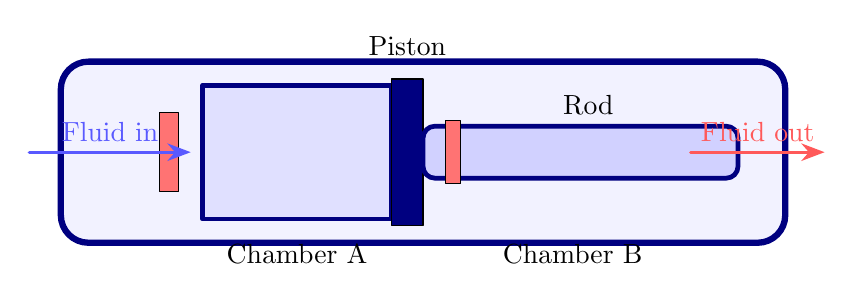
\begin{tikzpicture}[>=Stealth, line cap=round, line join=round]

\draw[fill=blue!5, draw=blue!50!black, line width=0.08cm, rounded corners=0.35cm] (1.2,3.2) rectangle (10.4,5.5);
\draw[fill=blue!12, draw=blue!50!black, line width=0.06cm] (3.0,3.5) rectangle (5.4,5.2);
\draw[fill=blue!50!black] (5.4,3.42) rectangle (5.8,5.28);
\draw[fill=blue!18, draw=blue!50!black, line width=0.06cm, rounded corners=0.15cm] (5.8,4.02) rectangle (9.8,4.68);
\draw[fill=red!55] (2.45,3.85) rectangle (2.7,4.85);
\draw[fill=red!55] (6.08,3.95) rectangle (6.28,4.75);
\draw[->, very thick, blue!65] (0.8,4.35) -- (2.85,4.35) node[midway, above] {Fluid in};
\draw[->, very thick, red!65] (9.2,4.35) -- (10.9,4.35) node[midway, above] {Fluid out};
\node[above] at (5.6,5.45) {Piston};
\node[above] at (7.9,4.7) {Rod};
\node[below] at (4.2,3.3) {Chamber A};
\node[below] at (7.7,3.3) {Chamber B};

      \end{tikzpicture}
      \end{document}
